\lipsum[1]

\subsection{Probe Requests}
A probe request consists of various information including, MAC address, device capabilities, sequence number, known hotspots etc.
Out of this we are interested in things which can identify a unique mobile device.
We collect the WiFi probe requests using the WireShark on hardware such as laptop for the pilot study and raspberry pi based custom sensor.
The Wi-Fi sensor collected all the probe requests which were broadcast around the area, and recorded the following data: the time-stamp at which they were collected, the MAC address of the source mobile device (anonymised using a hashing algorithm), the organisationally unique identifier (OUI) of the manufacturer of the device, the total length of the signal in bits, the strength of the signal reported by the mobile device in dBm, the sequence number of the signal, the duration for which the signal was transmitted, the service set identifier (SSID) of the access point targeted by the probe request, and the length of the extra information (tags) embedded in the packets.
	\begin{figure}
		\begin{center}
			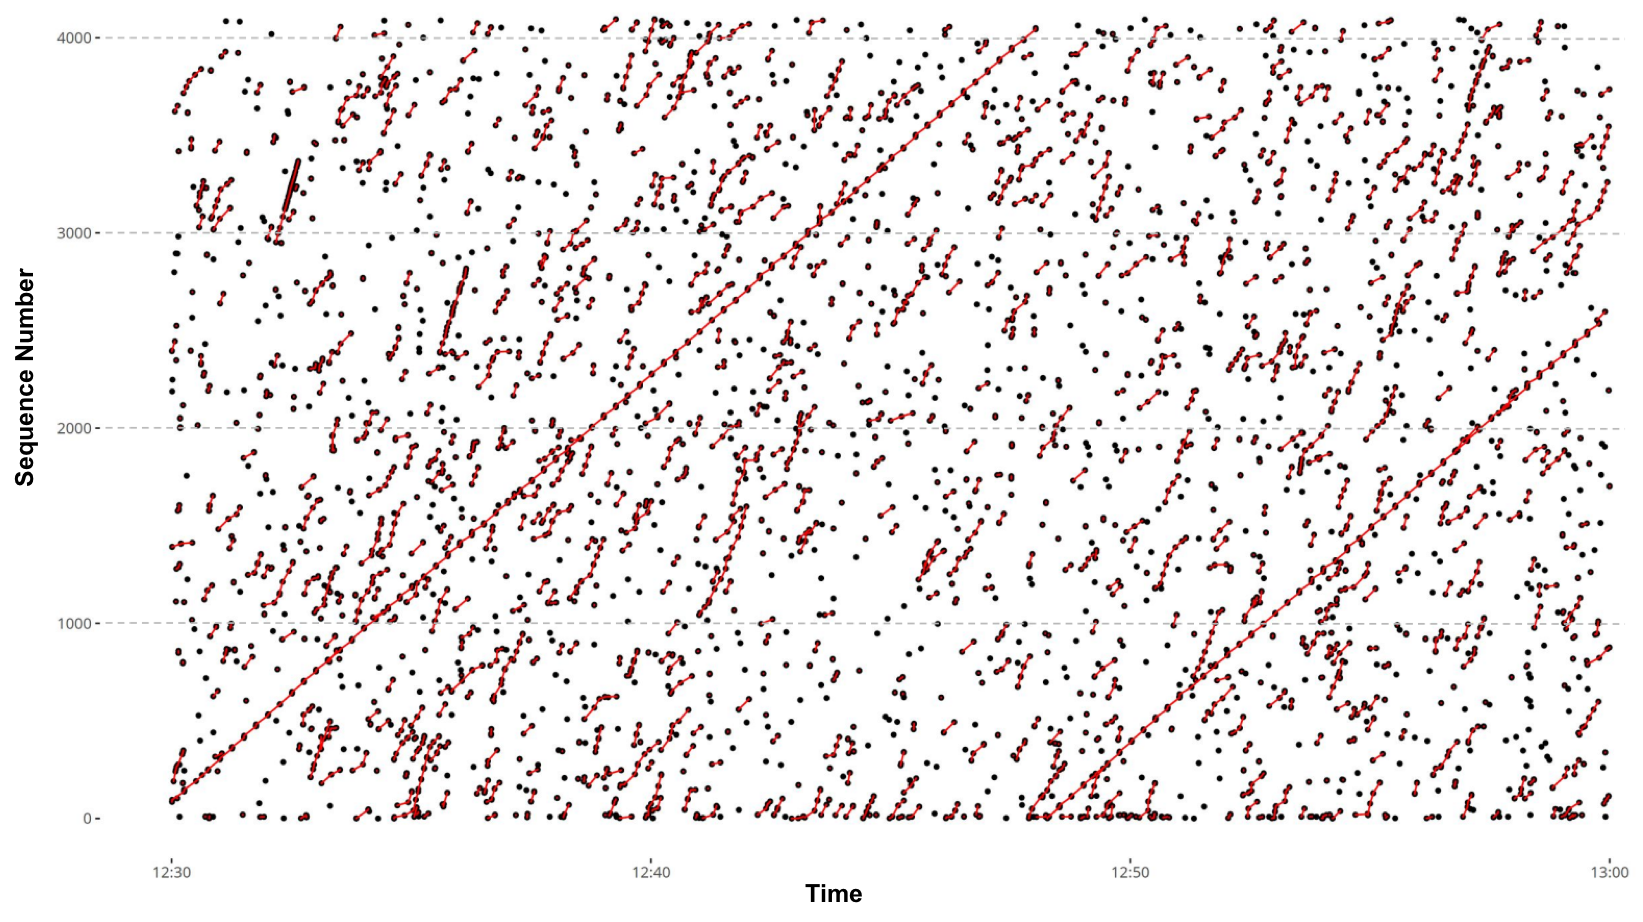
\includegraphics [width=\linewidth,trim=4 4 4 4,clip] {images/methodology_clustering.png}
			\caption{Clustering probe requests based on increasing sequence numbers present in them.}
			\label{clustering_pilot}
		\end{center}
	\end{figure}

\subsection{Data Collection}
The manual count was undertaken using an Android application on a mobile phone: the researcher touched the phone’s screen every time an individual pedestrian footfall was counted, and this was recorded as a time-stamp.
An initial analysis revealed that the fields - SSID and tags - were very sparse and did not provide much information for our cleaning process.
In addition, the duration field was closely related to the length of the probe request and provides no new information.
Therefore, we removed these fields from further analysis.
We eliminated the noise from devices outside the area of interest by removing all the probe requests which reported a "low" signal strength.
This classification of "high" vs "low" was performed using a k-means classification algorithm.
The cut-off point for the collected data was -71 dBm.
\subsection{Removing uncertainties}
\subsubsection{Signal Strength}
\lipsum[1-3]
\subsubsection{Device Fingerprinting}
We then used the fields - OUI, lengths and sequence number - to tackle the noise from devices which anonymised the probe requests.
OUI and length were used to split the dataset into groups of probe requests from similar devices, and each subset was classified further using a graph based clustering algorithm where each cluster corresponded to a unique device.
The algorithm created a graph where the probe requests represented the nodes, and links are created between them based on the following rules: 
	\begin{enumerate}
		\item A link could go only forward in time. 
		\item A link could exist between nodes with a maximum time difference of $\alpha$ (time threshold).
		\item A link could go from low to high sequence numbers.
		\item A link could exist between nodes with a maximum sequence number difference of $\beta$ (sequence threshold).
		\item A node could have only one incoming link and one outgoing link, which is the shortest of all such possible links.
	\end{enumerate}
The nodes were then classified based on the unique connected component they belonged to.
This classification was assigned as the unique identifier for the anonymised probe requests.
\subsubsection{Calibration}
\lipsum[1-2]
